\subsection{User interface} \label{cha:webinterface}
Users of the system has to be able to start the request and to see the data from the nodes when the request is complete. To make this a possibility, a user interface was created, which allows users to start requests, and see data from this and previous requests.

The interface runs as its own program, as a CGI (Common Gateway Interface) program running on the Raspberry Pi device, using Apache. The executable is located in \texttt{/usr/lib/cgi-bin/} and is called \texttt{WASP}. The program is written in C, and the complete code can be found in Appendix \ref{cha:uicode}.

When this program is run it prints out HTML, but because it is run as a CGI program using Apache, it is possible to connect to this program using a browser. When connected to the 'website', the user is able to make requests or show previous results. When a link is followed, a string is appended onto the current URL, for example \texttt{?request}. The string after the '?' is passed as an argument to the script.

On startup, the program attempts to fetch the process ID of the main node program, located in \texttt{/var/run/} if the program is running. This PID is used when the request button is presed by the user. The PID is necessary to call the procedure \texttt{kill}, that is used to signal the main node software that it should start a request. The signal is handled as explained in Chapter \ref{cha:signalhandling}.

When \texttt{kill} is issued, the program redirects to a waiting page. On this page, an AJAX request is performed every second to ping for a file in \texttt{/var/www/html/}. This ping will fail until the file \texttt{ping.txt} exists at this location. When the request is finished in the main node software, this file is created and the contents is set to the result name. When the file is written and closed by the main node software, the ping will succeed and the contents will be available. The browser can now be redirected to the result from the waiting screen. The ping file is then deleted as it is no longer needed.

The full sequence is shown on Figure \ref{fig:sigsequence}.
\begin{figure}[h!]
\centering
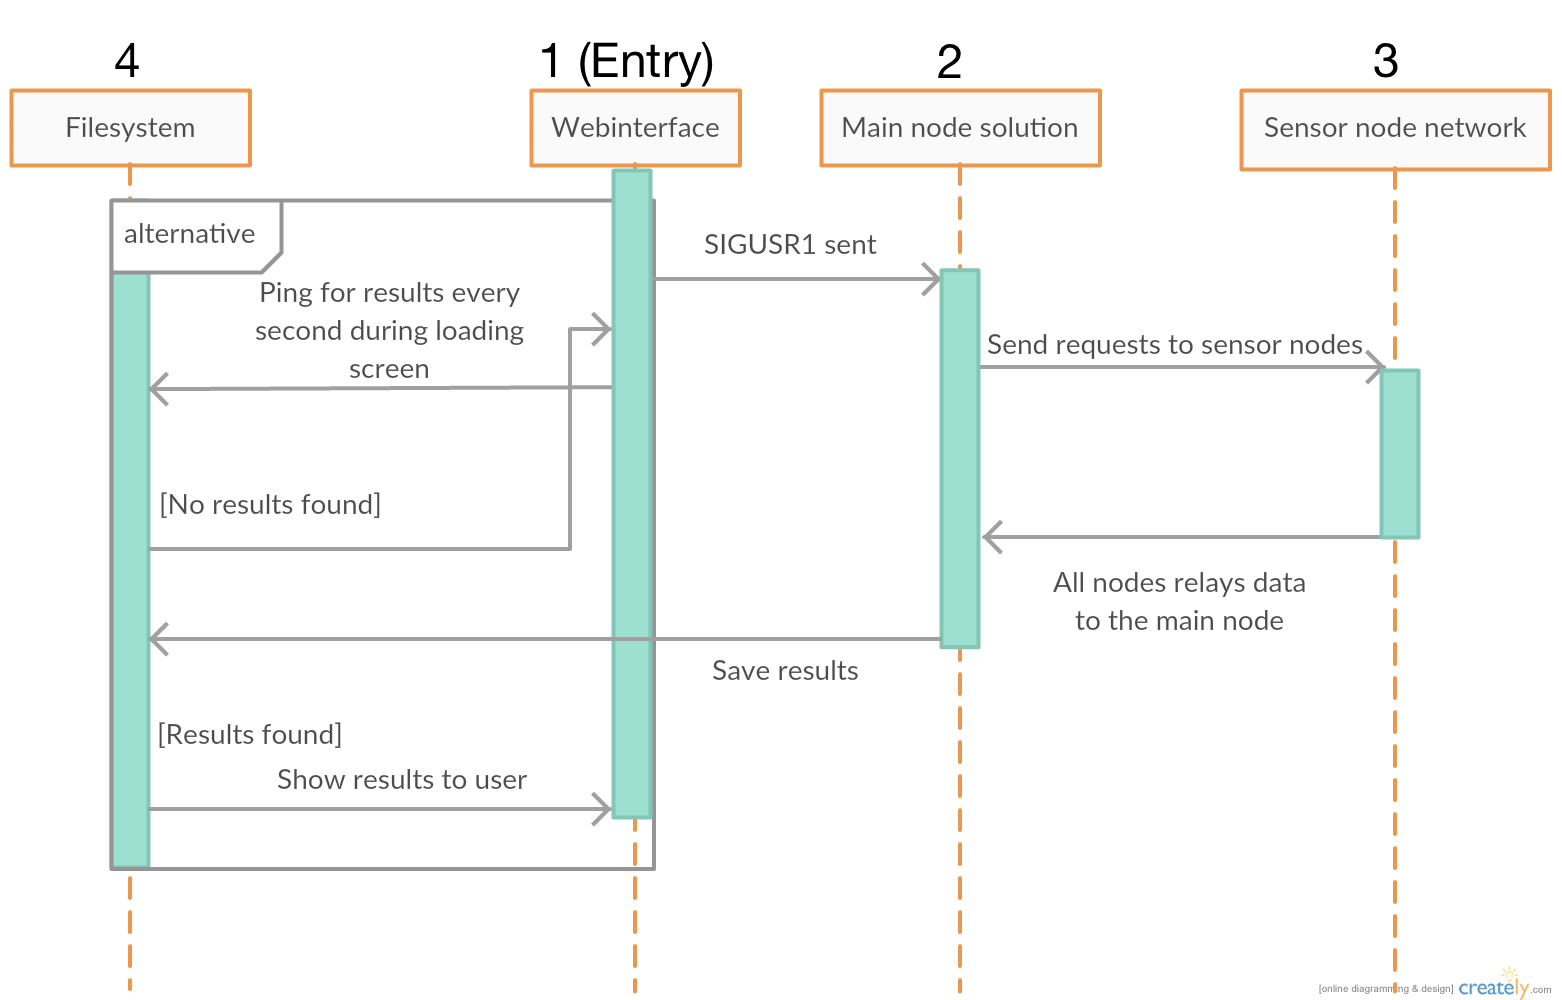
\includegraphics[width=1.1\textwidth]{chapters/implementation/figures/sigsequence.png}
\caption{Full sequence from webinterface to results\cite{creately}.}
\label{fig:sigsequence}
\end{figure}